% !TeX encoding = UTF-8
% !TeX program = pdflatex

\documentclass[11pt]{article}
\usepackage{graphicx}

\title{{\bf Diffie-Hellman for multiple parties} \\ \bigskip \large HW4 - CNS Sapienza}
\date{2018-11-23}
\author{Andrea Fioraldi 1692419}

\begin{document}
\maketitle

\section{Introduction}

Diffie-Hellman is one of the early methods for the exchanging of cryptographic keys in a public network. It was developed in 1976 \cite{Diffie1976} and now is a public domain algorithm.
An interesting result of 2015 \cite{Adrian2015a} shows that practical implementations of this method must not be considered secure against state actors.

In this report, we present a possible approach for the generalization of Diffie-Hellman (DH) for multiple parties and a consideration about the security of such a method.

\section{Classic DH Overview}

Before starting with the n-parties approach, we present a survey of the classic DH method between two parties.

We have two parties, Alice and Bob, that wants to share a key through a not secure channel.

The algorithm is the following:

\begin{itemize}
    \item Alice choose two numbers, $p$ and $g$. The first is a prime number, the second is the generator of the ciclyc multiplicative group $Z^*_p$, so every coprime of p can be expressed as a power of $g$ modulo $p$;
    \item Alice choose $a \in \{1, ..., p-1\}$ and compute $A = g^a$ $mod$ $p$;
    \item Alice sends $A$, $p$ and $g$ to Bob;
    \item Bob choose $b \in \{1, ..., p-1\}$ and compute $B = g^b$ $mod$ $p$;
    \item Bob sends $B$ to Alice;
    \item Now the two parts can compute a shared key $K = g^{ab}$ $mod$ $p$;
    \item Alice compute $K$ with $B^a$ $mod$ $p$;
    \item Bob compute $K$ with $A^b$ $mod$ $p$;
\end{itemize} 

\begin{figure}[!ht]
    \centering
    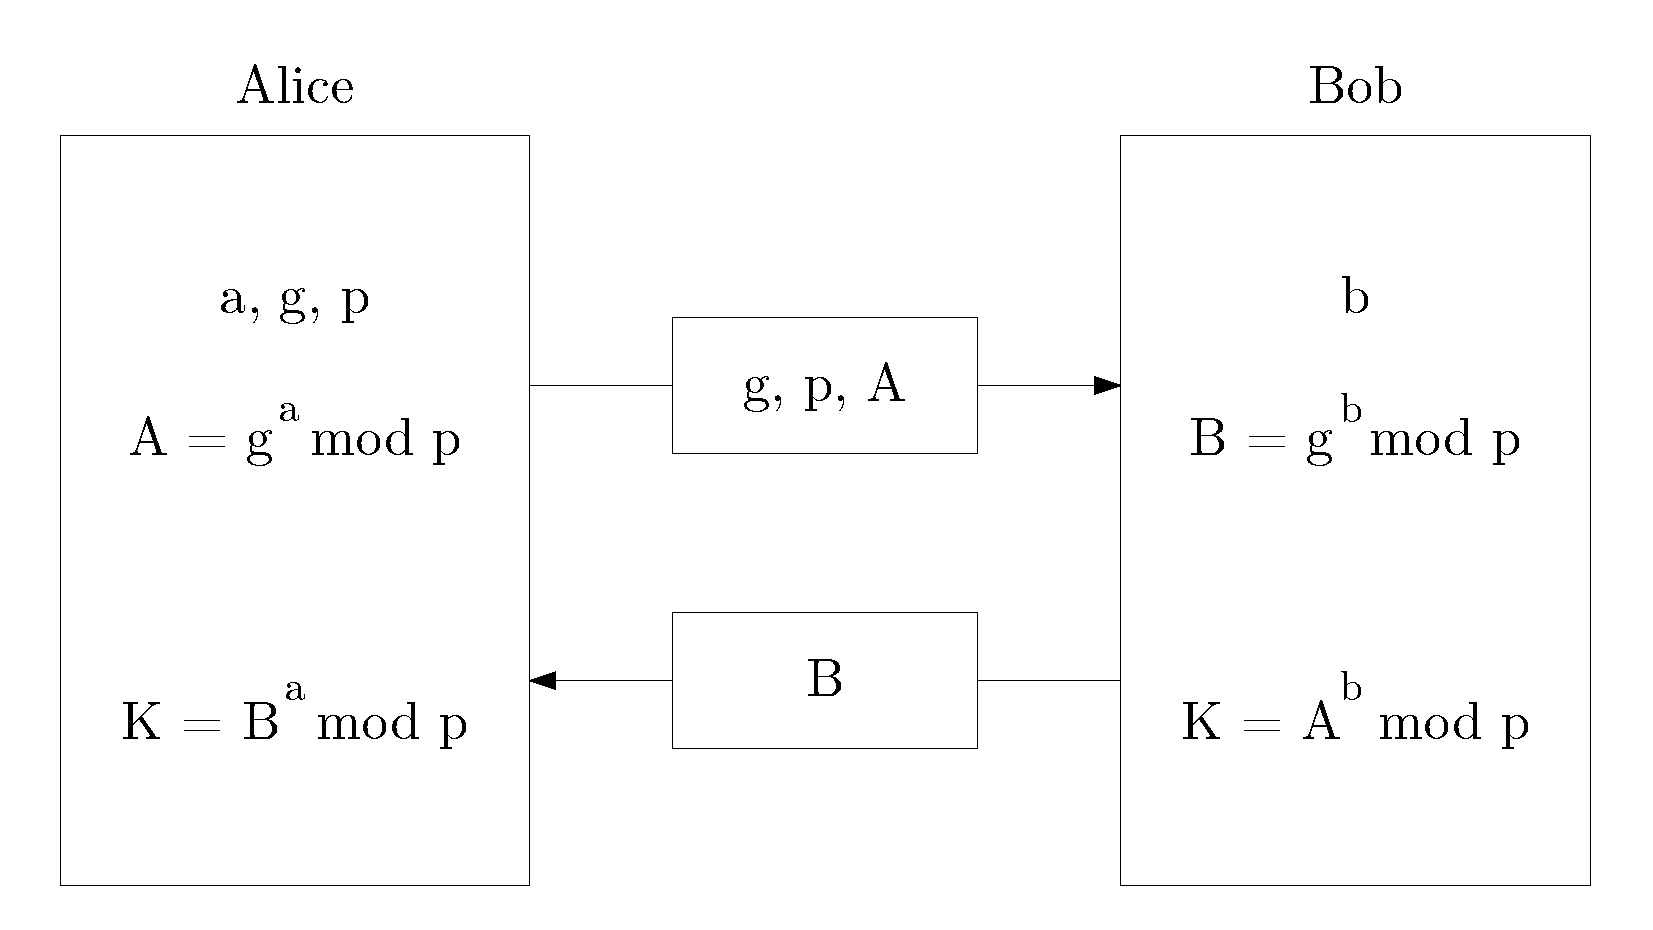
\includegraphics[width=1\textwidth]{dhimg-hw4-1692419}
    \caption{DH Key exchange schema}
    \label{fig:dhimg}
\end{figure}

The shared key $K$ can be further used in a communication based on a symmetric encryption like AES. 

\subsection{Security}

A DH key is considered secure due to the fact that it is not distinguishable from random bytes in polynomial time thanks to the fact that computing $x$ given $g^x$ ($g$ is a generator as said before) is almost as hard as the discrete logarithm problem \cite{discrete}.
Reversing such one-way function is possible only with a brute-force, so with a large $x$ this process is computationally infeasible. An attacker can get both the $A$ and $B$ keys of Alice and Bob but can't compute the shared key $K$.
However, DH is vulnerable to main in the middle. An attacker can impersonate Alice when communicating with Bob and vice-versa. In this case, the attacker is not computing the secret numbers of Alice and Bob but is generating two pairs of secrets for the two parties and performing DH (like a proxy). So, in the end, the attacker has two shared key, one for the communication with Alice and one for Bob.

\section{Three parties DH}

We start presenting multi-parties DH in a case with three parties and then we will expose a generalization for n-parties.

The parties are Alice, Bob, and Woody. In the selected approach, proposed in 2008 in \cite{Biswas}, one of the parties is a master that establish the key and then become a normal user. In our example the master is Alice.

The method proceeds in the following way:

\begin{itemize}
    \item Alice choose two numbers, $p$ and $g$, as in classic DH.
    \item Alice choose $a \in \{1, ..., p-1\}$ and compute $A = g^a$ $mod$ $p$;
    \item Alice sends $A$, $p$ and $g$ to Bob and Woody;
    \item Bob choose $b \in \{1, ..., p-1\}$ and compute $B = g^b$ $mod$ $p$;
    \item Bob sends $B$ to Alice;
    \item Woody choose $c \in \{1, ..., p-1\}$ and compute $C = g^c$ $mod$ $p$;
    \item Woody sends $C$ to Alice;
    \item Now two shared keys can be computet, $K_b = g^{ab}$ $mod$ $p$ and $K_c = g^{ac}$ $mod$ $p$;
    \item Alice compute both keys with $K_b = B^a$ $mod$ $p$ and $K_c = C^a$ $mod$ $p$;
    \item Bob compute $K_b$ with $A^b$ $mod$ $p$;
    \item Woody compute $K_c$ with $A^c$ $mod$ $p$;
    \item Alice compute $D_c = g^{K_c}$ $mod$ $p$ and sends it to Bob;
    \item Alice compute $D_b = g^{K_b}$ $mod$ $p$ and sends it to Woody;
    \item Bob compute $K = (D_c)^{K_b}$ $mod$ $p = g^{K_b*K_c}$ $mod$ $p$;
    \item Woody compute $K = (D_b)^{K_c}$ $mod$ $p = g^{K_b*K_c}$ $mod$ $p$;
    \item Alice compute $K = g^{K_b*K_c}$ $mod$ $p$ directly;
    \item Now all parties share the key $K$ and Alice is not a master anymore.
\end{itemize}

The steps involving Bob and Woody can be in parallel. The master performs $n$ exponentiations so the overall performance is based on $P_i$. Thus, for a better implementation between machines is good to elect as master the machine with the highest computational power.

\section{Multi parties DH}

In this section we present the generalization of the previous exposed approach on $n$ parties, $P_i$ with $i \in \{1, ..., n\}$. In this case we select as master $P_i$ and the other parties, $P_j$ with $j \neq i$, are slaves.

\begin{itemize}
    \item $P_i$ choose two numbers, $p$ and $g$, as in classic DH.
    \item $P_i$ choose $x_i \in \{1, ..., p-1\}$ and compute $X_i = g^{x_i}$ $mod$ $p$;
    \item $P_i$ sends $X_i$, $p$ and $g$ to the other parties $P_j$;
    \item Each $P_j$ choose an $x_j \in \{1, ..., p-1\}$ and compute $X_j = g^{x_j}$ $mod$ $p$;
    \item Each $P_j$ sends $X_j$ to $P_i$;
    \item Each $P_j$ generates a key $K_j = (X_i)^{x_j}$ $mod$ $p = g^{x_i*x_j}$ $mod$ $p$;
    \item $P_i$ generates $n-1$ keys for each slave $P_j$, $K_j = (X_j)^{x_i}$ $mod$ $p = g^{x_i*x_j}$ $mod$ $p$;
    \item $P_i$, for all slaves, combines all generated keys in $X_{k,j} = g^{\Pi K_{k \neq j} }$ $mod$ $p$;
    \item $P_i$, for all slaves, sends $X_{k,j}$ to the correspondent $P_j$;
    \item Each $P_j$ compute the final key $K = (X_{k,j})^{K_j}$ $mod$ $p = g^{K_1,...,K_n}$ $mod$ $p$;
    \item $P_i$ compute directly the final key $K = g^{K_1,...,K_n}$ $mod$ $p$;
    \item Now all parties share the key $K$ and $P_i$ is not a master anymore.
\end{itemize}

The method is synchronous for $P_i$ and $P_j$ ($j \neq i$) but all the $P_j$ parties work asynchronously and do not need to know the number of the parties.

\section{Security considerations}

The proposed multi-parties method final key, $K$, is not distinguishable in polynomial time from random numbers. This is true because the generation of the public keys in the first stage, $X_i$ $i \in \{1, ..., n\}$, follows the standard DH protocol and the generation fo $K$ follows an equivalent procedure of DH because it is an exponentiation of a product of secret values instead of a single secret value.

As standard DH, this method is vulnerable to man in the middle. If an attacker compromise a slave $P_j$ it can control only the communication between 

\vfill

\begin{thebibliography}{99}

\bibitem{Diffie1976}
W.~Diffie and M.~E. Hellman, ``New directions in cryptography,'' {\em IEEE
  Trans.\ Info.\ Theory}, vol.~22, pp.~644--54, November 1976.

\bibitem{Adrian2015a}
D.~Adrian, K.~Bhargavan, Z.~Durumeric, P.~Gaudry, M.~Green, J.~A. Halderman,
  N.~Heninger, D.~Springall, E.~Thom\'{e}, L.~Valenta, B.~VanderSloot,
  E.~Wustrow, S.~Zanella-B'{e}guelin, and P.~Zimmermann, ``Imperfect forward
  secrecy: How {Diffie--Hellman} fails in practice,'' in {\em CCS'15}, (Denver,
  Colorado), October 12--16, 2015.

\bibitem{discrete}
``{Discrete logarithm - Wikipedia}.'' \verb|https://en.wikipedia.org/wiki/Discrete_logarithm|.
\newblock Accessed: 2018-11-26.

\bibitem{Biswas}
G.~P. Biswas, ``Diffie-hellman technique: extended to multiple two-party keys
  and one multi-party key,'' {\em IET Information Security}, vol.~2,
  pp.~12--18, March 2008.


\end{thebibliography}

\end{document}
